
\documentclass{beamer} 


\mode<presentation>
{
  \usetheme{Berkeley}
  % or ...

  \setbeamercovered{transparent}
  % or whatever (possibly just delete it)
}

\usepackage{tikz}
\usepackage{graphicx}
\usepackage[english]{babel}
% or whatever

\usepackage[utf8]{inputenc}
% or whatever

\usepackage{times}
\usepackage[T1]{fontenc}
% Or whatever. Note that the encoding and the font should match. If T1
% does not look nice, try deleting the line with the fontenc.


\title[Research Transparency in the Social Sciences] % (optional, use only with long paper titles)
{Research Transparency in the Social Sciences}

\subtitle
{}

\author[Christensen] % (optional, use only with lots of authors)
{Garret~Christensen\inst{1}}
% - Give the names in the same order as the appear in the paper.
% - Use the \inst{?} command only if the authors have different
%   affiliation.

\institute[Universities of Somewhere and Elsewhere] % (optional, but mostly needed)
{
  \inst{1}%
  UC Berkeley:\\
  Berkeley Initiative for Transparency in the Social Sciences\\
  Berkeley Institute for Data Science\\
  }
% - Use the \inst command only if there are several affiliations.
% - Keep it simple, no one is interested in your street address.

\date[BITSS2014] % (optional, should be abbreviation of conference name)
{World Bank, February 2017\\
Slides available online at \url{http://www.github.com/BITSS/WorldBankFeb2017}}
% - Either use conference name or its abbreviation.
% - Not really informative to the audience, more for people (including
%   yourself) who are reading the slides online

\subject{Research Transparency}
% This is only inserted into the PDF information catalog. Can be left
% out. 

\pgfdeclareimage[height=2cm]{university-logo}{../Images/BITSSlogo.png}
\logo{\pgfuseimage{university-logo}}

% If you have a file called "university-logo-filename.xxx", where xxx
% is a graphic format that can be processed by latex or pdflatex,
% resp., then you can add a logo as follows:

% \pgfdeclareimage[height=0.5cm]{university-logo}{university-logo-filename}
% \logo{\pgfuseimage{university-logo}}



% Delete this, if you do not want the table of contents to pop up at
% the beginning of each subsection:
%\AtBeginSubsection[]
%{
%  \begin{frame}<beamer>{Outline}
%    \tableofcontents[currentsection,currentsubsection]
%  \end{frame}
%}


% If you wish to uncover everything in a step-wise fashion, uncomment
% the following command: 

\beamerdefaultoverlayspecification{<.->}


\begin{document}

\begin{frame}
  \titlepage
\end{frame}




% Structuring a talk is a difficult task and the following structure
% may not be suitable. Here are some rules that apply for this
% solution: 

% - Exactly two or three sections (other than the summary).
% - At *most* three subsections per section.
% - Talk about 30s to 2min per frame. So there should be between about
%   15 and 30 frames, all told.

% - A conference audience is likely to know very little of what you
%   are going to talk about. So *simplify*!
% - In a 20min talk, getting the main ideas across is hard
%   enough. Leave out details, even if it means being less precise than
%   you think necessary.
% - If you omit details that are vital to the proof/implementation,
%   just say so once. Everybody will be happy with that.
%%%%%%%%%%%%%%%%%%%%%%%%%%%%%%%%%%%%%%%%%%%%%%%%%%%%%%%%%%%%%%%%%%%%%%%
%%%%%%%%%%%%%%%%%%%%%%%%%%%%%%%%%%%%%%%%%%%%%%%%%%%%%%%%%%%%%%%%%%%%%
\begin{frame}{Outline}
  \tableofcontents
  % You might wish to add the option [pausesections]
\end{frame}
\section {Introduction}
{ % all template changes are local to this group.
    \setbeamertemplate{navigation symbols}{}
    \begin{frame}[plain]
        \begin{tikzpicture}[remember picture,overlay]
            \node[at=(current page.center)] {
                \href{https://www.bitss.org/}{\includegraphics[width=\paperwidth]{../Images/bitsslogo.png}}
            };
        \end{tikzpicture}
     \end{frame}
}

{ % all template changes are local to this group.
    \setbeamertemplate{navigation symbols}{}
    \begin{frame}[plain]
        \begin{tikzpicture}[remember picture,overlay]
            \node[at=(current page.center)] {
                \href{https://www.bitss.org/}{
\includegraphics[width=\paperwidth]{../Images/ecosystem.PNG}}
            };
        \end{tikzpicture}
     \end{frame}
}
%%%%%%%%%%%%%%%%%%%%%%%%%%%%%%%%%%%%%%%%%%%%%%%%%%%%%%%%%%%%%%%%%%%%%%%%%%%%%%%%%%%
\section{Ethical Research}
\begin{frame}{Ethical Research}
\begin{itemize}
\item Transparency is part of being an ethical researcher. 

\item Scientific values espoused by Robert Merton (Merton 1942):
\begin{itemize}[<.->]
\item Universalism: anyone can make a claim regardless of status.
\item Communism: open sharing of knowledge.
\item Disinterestedness: truth as motivation, not financial gains (COI).
\item Organized skepticism: peer review, replication.
\end{itemize}
\end{itemize}
\end{frame}

\begin{frame}{Ethical Research}
\begin{itemize}
\item
Fraud exists \href{http://pss.sagepub.com/content/24/10/1875}{(Simonsohn 2013)}, but mostly we should admit that we're human, subject to bias and motivated reasoning, transparency can help with this \href{http://pps.sagepub.com/content/7/6/615.short}{(Nosek, Spies, Motyl 2012)}.
\item
Those of us who run experiments or use data with personal identifying information should take IRBs seriously as part of transparency (Ch. 11--13 Morton \& Williams 2010, \href{http://desposato.org/ethicsfieldexperiments.pdf}{Desposato 2014}). 
\end{itemize}
\end{frame}

%{ % all template changes are local to this group.
%    \setbeamertemplate{navigation symbols}{}
%    \begin{frame}[plain]
%        \begin{tikzpicture}[remember picture,overlay]
%            \node[at=(current page.center)] {
%                
\includegraphics[height=\paperheight]{../Images/motivatedreasoning.PNG}
%            };
%        \end{tikzpicture}
%     \end{frame}
%}
%{ % all template changes are local to this group.
%    \setbeamertemplate{navigation symbols}{}
%    \begin{frame}[plain]
%        \begin{tikzpicture}[remember picture,overlay]
%            \node[at=(current page.center)] {
%                \href{http://www.nytimes.com/2014/10/29/upshot/professors-research-project-%stirs-political-outrage-in-montana.html}{
\includegraphics[width=\paperwidth]{../Images/Montana1.PNG}}
%            };
%        \end{tikzpicture}
%     \end{frame}
%}
%{ % all template changes are local to this group.
%    \setbeamertemplate{navigation symbols}{}
%    \begin{frame}[plain]
%        \begin{tikzpicture}[remember picture,overlay]
%            \node[at=(current page.center)] {
%                \href{https://www.washingtonpost.com/news/monkey-cage/wp/2015/05/13/campaign-experiment-found-to-be-in-violation-of-montana-law/}{
\includegraphics[width=\paperwidth]{../Images/Montana2.PNG}}
%            };
%        \end{tikzpicture}
%     \end{frame}
%}

%HERE'S THE BASIC SYNTAX TO SHOW FIGURE AND IMAGE ON SAME SLIDE
%\begin{frame}
%Why we worry: \href{http://pss.sagepub.com/content/23/5/524}{(John, Loewenstein, Prelec 2011)}
%\frame{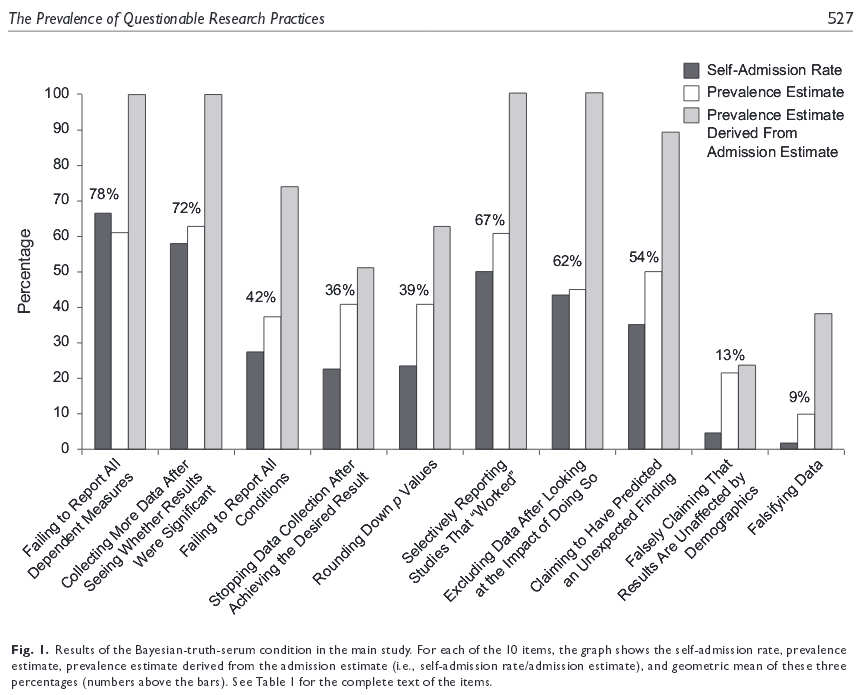
\includegraphics[scale=0.375]{../Images/PrelecFig1.PNG}}
%\end{frame}

\begin{frame}{Ethical Research}
Why we worry:
\begin{itemize}[<.->]
\item \href{http://www.jstor.org/stable/pdf/10.1525/jer.2007.2.4.3.pdf}{(Anderson, Martinson, De Vries 2007)}
\item \href{http://pss.sagepub.com/content/23/5/524}{(John, Loewenstein, Prelec 2011)}
\end{itemize}
\end{frame}

{ % all template changes are local to this group.
    \setbeamertemplate{navigation symbols}{}
    \begin{frame}[plain]
        \begin{tikzpicture}[remember picture,overlay]
            \node[at=(current page.center)] {
                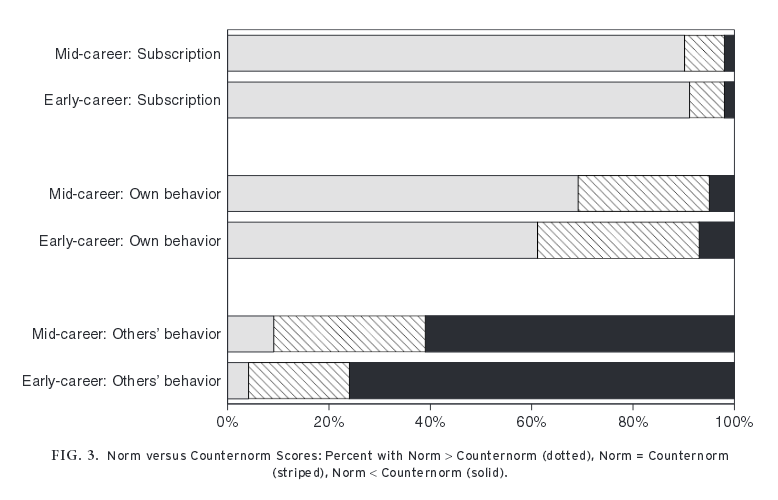
\includegraphics[width=\paperwidth]{../Images/AMdV2007.PNG}
            };
        \end{tikzpicture}
     \end{frame}
}
{ % all template changes are local to this group.
    \setbeamertemplate{navigation symbols}{}
    \begin{frame}[plain]
        \begin{tikzpicture}[remember picture,overlay]
            \node[at=(current page.center)] {
                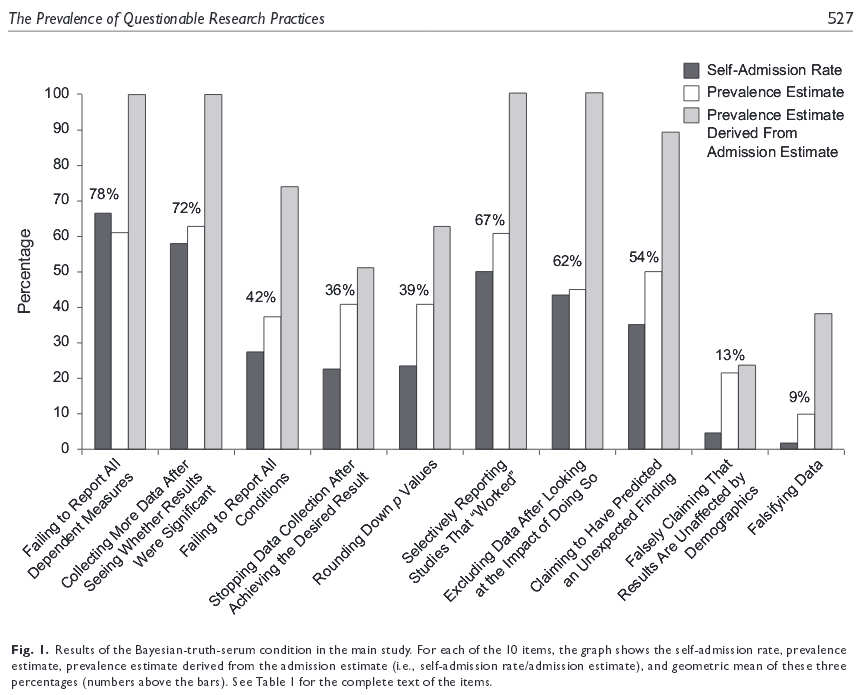
\includegraphics[height=\paperheight]{../Images/PrelecFig1.PNG}
            };
        \end{tikzpicture}
     \end{frame}
}

%\end{frame}
%%%%%%%%%%%%%%%%%%%%%%%%%%%%%%%%%%%%%%%%%%%%%%%%%%%%%%%%%%%%%%%%%%
%\section{Study Design and Power}
%\begin{frame}{Study Design and Power}
%\begin{itemize}[<.->]
%\item
%Adequately power trials to help prevent spurious significant results. 
%\item
%Practical suggestions:
%\begin{itemize}
%\item
%Collaborate with other labs to mutually run each others' experiments (Open Science Collaboration 2014, 2015).
%\begin{itemize}[<.->]
%\item \href{http://science.sciencemag.org/content/349/6251/aac4716.full}{Replication Project: Psychology}
%\item \href{http://econtent.hogrefe.com/doi/full/10.1027/1864-9335/a000178}{Many Labs 1}, \href{https://osf.io/8cd4r/}{2}, 3
%\item Crowdsourcing Analysis \href{http://www.nature.com/news/crowdsourced-research-many-hands-make-tight-work-1.18508}{(Silberzahn and Uhlmann 2016)}
%\item \href{http://science.sciencemag.org/content/early/2016/03/02/science.aaf0918}{Experimental economics replications (Camerer et al. 2016)}
%\end{itemize}
%\item
%Maximize power subject to budget constraint by adjusting expensive treatment arm (relative) size \href{http://citeseerx.ist.psu.edu/viewdoc/download?doi=10.1.1.650.9734&rep=rep1&type=pdf}{(Duflo, Glennerster, Kremer 2007)}. 
%\end{itemize}
%\end{itemize}
%\end{frame}

%{ % all template changes are local to this group.
%    \setbeamertemplate{navigation symbols}{}
%    \begin{frame}[plain]
%        \begin{tikzpicture}[remember picture,overlay]
%            \node[at=(current page.center)] {
%                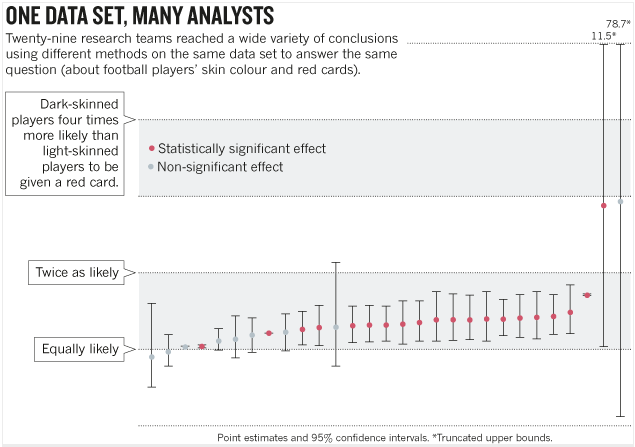
\includegraphics[width=\paperwidth]{../Images/Crowdsourcing2.PNG}
%            };
%        \end{tikzpicture}
%     \end{frame}
%}
%%%%%%%%%%%%%%%%%%%%%%%%%%%%%%%%%%%%%%%%%%%%%%%%%%%%%%%%%%%%%%%%%%%%%
\section{Registrations}

\subsection*{Publication Bias}
\begin{frame}{Publication Bias}%{Subtitles are optional.}
  % - A title should summarize the slide in an understandable fashion
  %   for anyone how does not follow everything on the slide itself.
  Existence of the problem:
  \begin{itemize}
  \item
 Effect sizes diminish with sample size (\href{http://pan.oxfordjournals.org/content/9/4/385.short}{Gerber, Green, Nickerson 2001})
  \item
  There is a higher fraction of rejected hypothesis tests in social compared to hard sciences (\href{http://journals.plos.org/plosone/article?id=10.1371/journal.pone.0010068}{Fanelli 2010}).
  \item
  	Published null results are disappearing over time, in all disciplines (\href{http://link.springer.com/article/10.1007/s11192-011-0494-7}{Fanelli 2011}). 
  \item
  	Data on the complete set of experiments run shows strong results are 40pp more likely to be published, and 60pp more likely to be written up. The file drawer problem is large. (\href{http://science.sciencemag.org/content/345/6203/1502}{Franco, Malhotra, Simonovits 2014})
  \end{itemize}
\end{frame}

%Go through the fields

\begin{frame}{All Fields}
\begin{itemize}[<.->]
\item Medicine: \href{http://www.nejm.org/doi/full/10.1056/nejmsa065779}{(Turner et al. 2008)}
\item Social Sciences: \href{http://science.sciencemag.org/content/345/6203/1502.short}{(Franco, Malhotra, Simonovits 2014)}
\item Economics: \href{https://www.aeaweb.org/articles.php?doi=10.1257/app.20150044}{(Brodeur et al. 2016)}
\item Sociology: \href{http://smr.sagepub.com/content/37/1/3.short}{(Gerber and Malhotra 2008)}
\item Political Science: \href{http://nowpublishers.com/article/Details/QJPS-8024}{(Gerber and Malhotra 2008)}
\end{itemize}
\end{frame}

{ % all template changes are local to this group.
    \setbeamertemplate{navigation symbols}{}
    \begin{frame}[plain]
        \begin{tikzpicture}[remember picture,overlay]
            \node[at=(current page.center)] {
                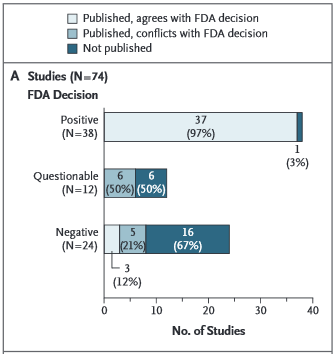
\includegraphics[height=\paperheight]{../Images/TurnerFigure1.PNG}
            };
        \end{tikzpicture}
     \end{frame}
}
{ % all template changes are local to this group.
    \setbeamertemplate{navigation symbols}{}
    \begin{frame}[plain]
        \begin{tikzpicture}[remember picture,overlay]
            \node[at=(current page.center)] {
                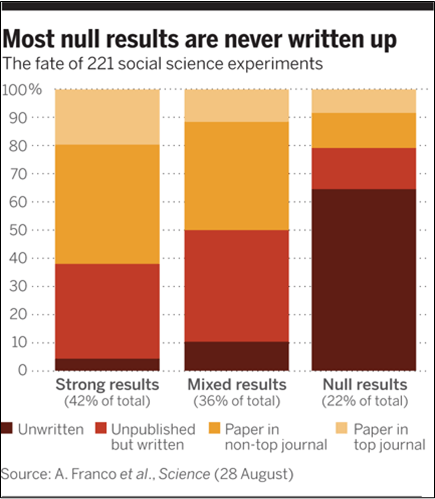
\includegraphics[height=\paperheight]{../Images/Tess.PNG}
            };
        \end{tikzpicture}
     \end{frame}
}
{ % all template changes are local to this group.
    \setbeamertemplate{navigation symbols}{}
    \begin{frame}[plain]
        \begin{tikzpicture}[remember picture,overlay]
            \node[at=(current page.center)] {
                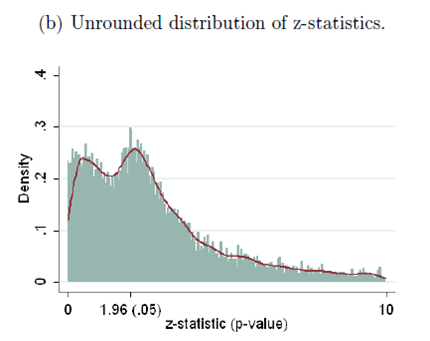
\includegraphics[height=\paperheight]{../Images/Brodeur.PNG}
            };
        \end{tikzpicture}
     \end{frame}
}
{ % all template changes are local to this group.
    \setbeamertemplate{navigation symbols}{}
    \begin{frame}[plain]
        \begin{tikzpicture}[remember picture,overlay]
            \node[at=(current page.center)] {
                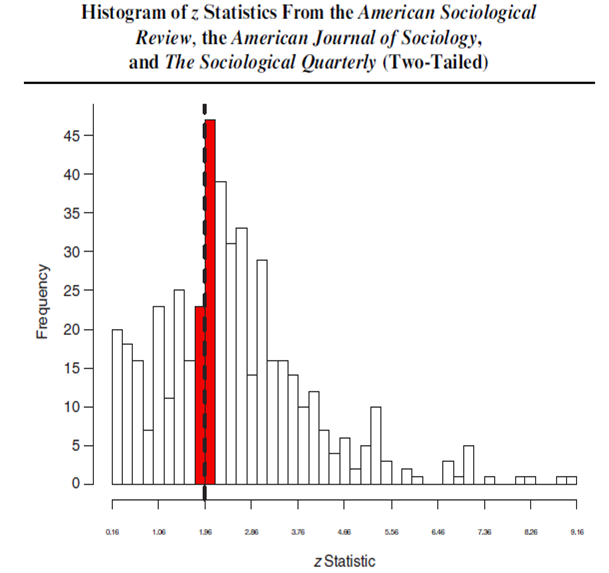
\includegraphics[height=\paperheight]{../Images/GerberSoc.PNG}
            };
        \end{tikzpicture}
     \end{frame}
}
{ % all template changes are local to this group.
    \setbeamertemplate{navigation symbols}{}
    \begin{frame}[plain]
        \begin{tikzpicture}[remember picture,overlay]
            \node[at=(current page.center)] {
                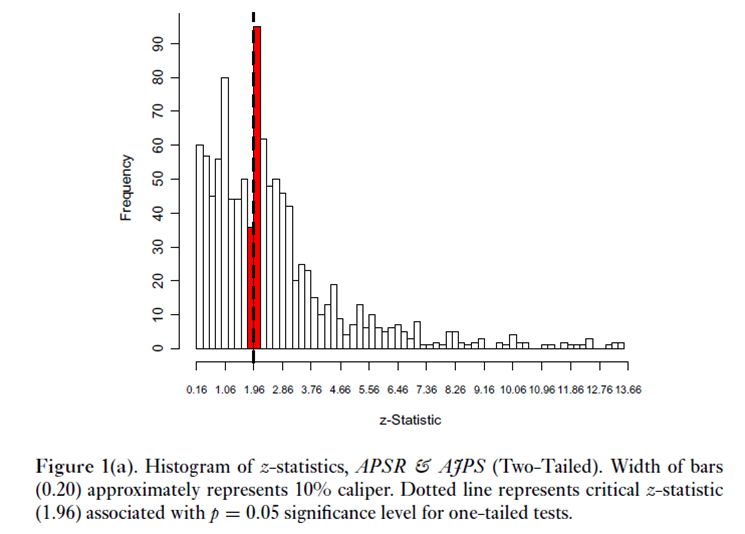
\includegraphics[height=\paperheight]{../Images/GerberPS.PNG}
            };
        \end{tikzpicture}
     \end{frame}
}




\begin {frame}{Publication Bias}
If we only write up/publish significant results, and we have no record of all the insignificant results, we have no way to tell if our `significant' results are real, or if they're the 5\% we should expect due to noise.
\end{frame}

\subsection*{Registrations}
\begin{frame}{Registration}
Registration as Solution to Publication Bias:
 \begin{itemize}
  \item
   Publicly stating all research you will do, what hypotheses you will test, prospectively.
   %\item If we know every hypothesis test that is run on a given subject, we have a better idea of how seriously to take the significant results.
  \item
   Near universal adoption in medical RCTs. Top journals (ICMJE) won't publish if it's not registered. \url{http://clinicaltrials.gov}
  \item
   Even better if registry requires outcomes from after study. Currently limited, but NIH is moving on this.
\end{itemize}
\end{frame}

\begin{frame}{Registration}
 Newer to social sciences, but:
   \begin{itemize}[<.->]
   \item
   	AEA registry, currently only for RCTs. \url{http://socialscienceregistry.org}
   \item
    EGAP registry \url{http://egap.org/design-registration}
   \item 
    3ie registry, for developing country evaluations. \url{http://ridie.3ieimpact.org}
   \item
   	Open Science Framework\\ \url{http://osf.io}
   	\begin{itemize}
   	\item
   	Open format
   	\item
   	Will soon sync with above
   	\end{itemize}
   	\item Simple: \url{http://aspredicted.org}
   \end{itemize}
 
\end{frame}

 { % all template changes are local to this group.
    \setbeamertemplate{navigation symbols}{}
    \begin{frame}[plain, label=AEAreg]
         \begin{tikzpicture}[remember picture,overlay]
            \node[at=(current page.center)] {
                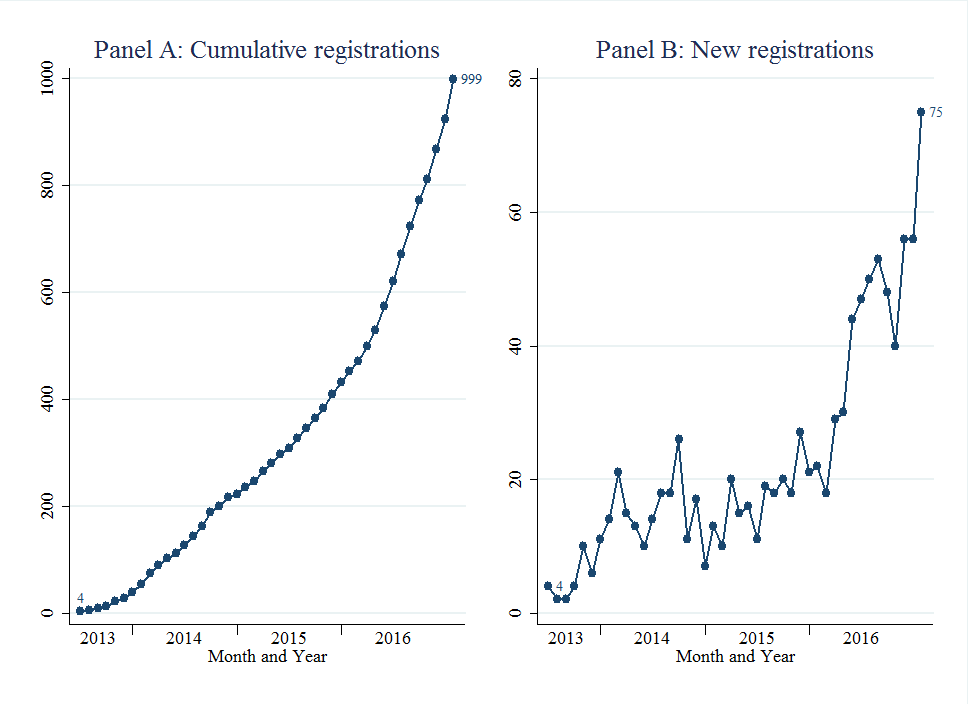
\includegraphics[height=\paperheight]{../Images/combinedAEARegGraphs.PNG}
            };
        \end{tikzpicture}
     \end{frame}
}

\begin{frame}{Design-Based Publication}
AKA Registered Reports, moves peer review before data gathering, results, and analysis.

\begin{enumerate}[<.->]
\item Design a project
\item Submit
\item Reviewed based on importance of question and quality of design
\item Get in-principle acceptance
\item Follow through, and nulls get published
\end{enumerate}
\href{https://osf.io/8mpji/wiki/home/}{20 Journals, 5 more with Special Issues \beamergotobutton{Link}}
\end{frame}

{ % all template changes are local to this group.
    \setbeamertemplate{navigation symbols}{}
    \begin{frame}[plain, label=AEAreg]
         \begin{tikzpicture}[remember picture,overlay]
            \node[at=(current page.center)] {
                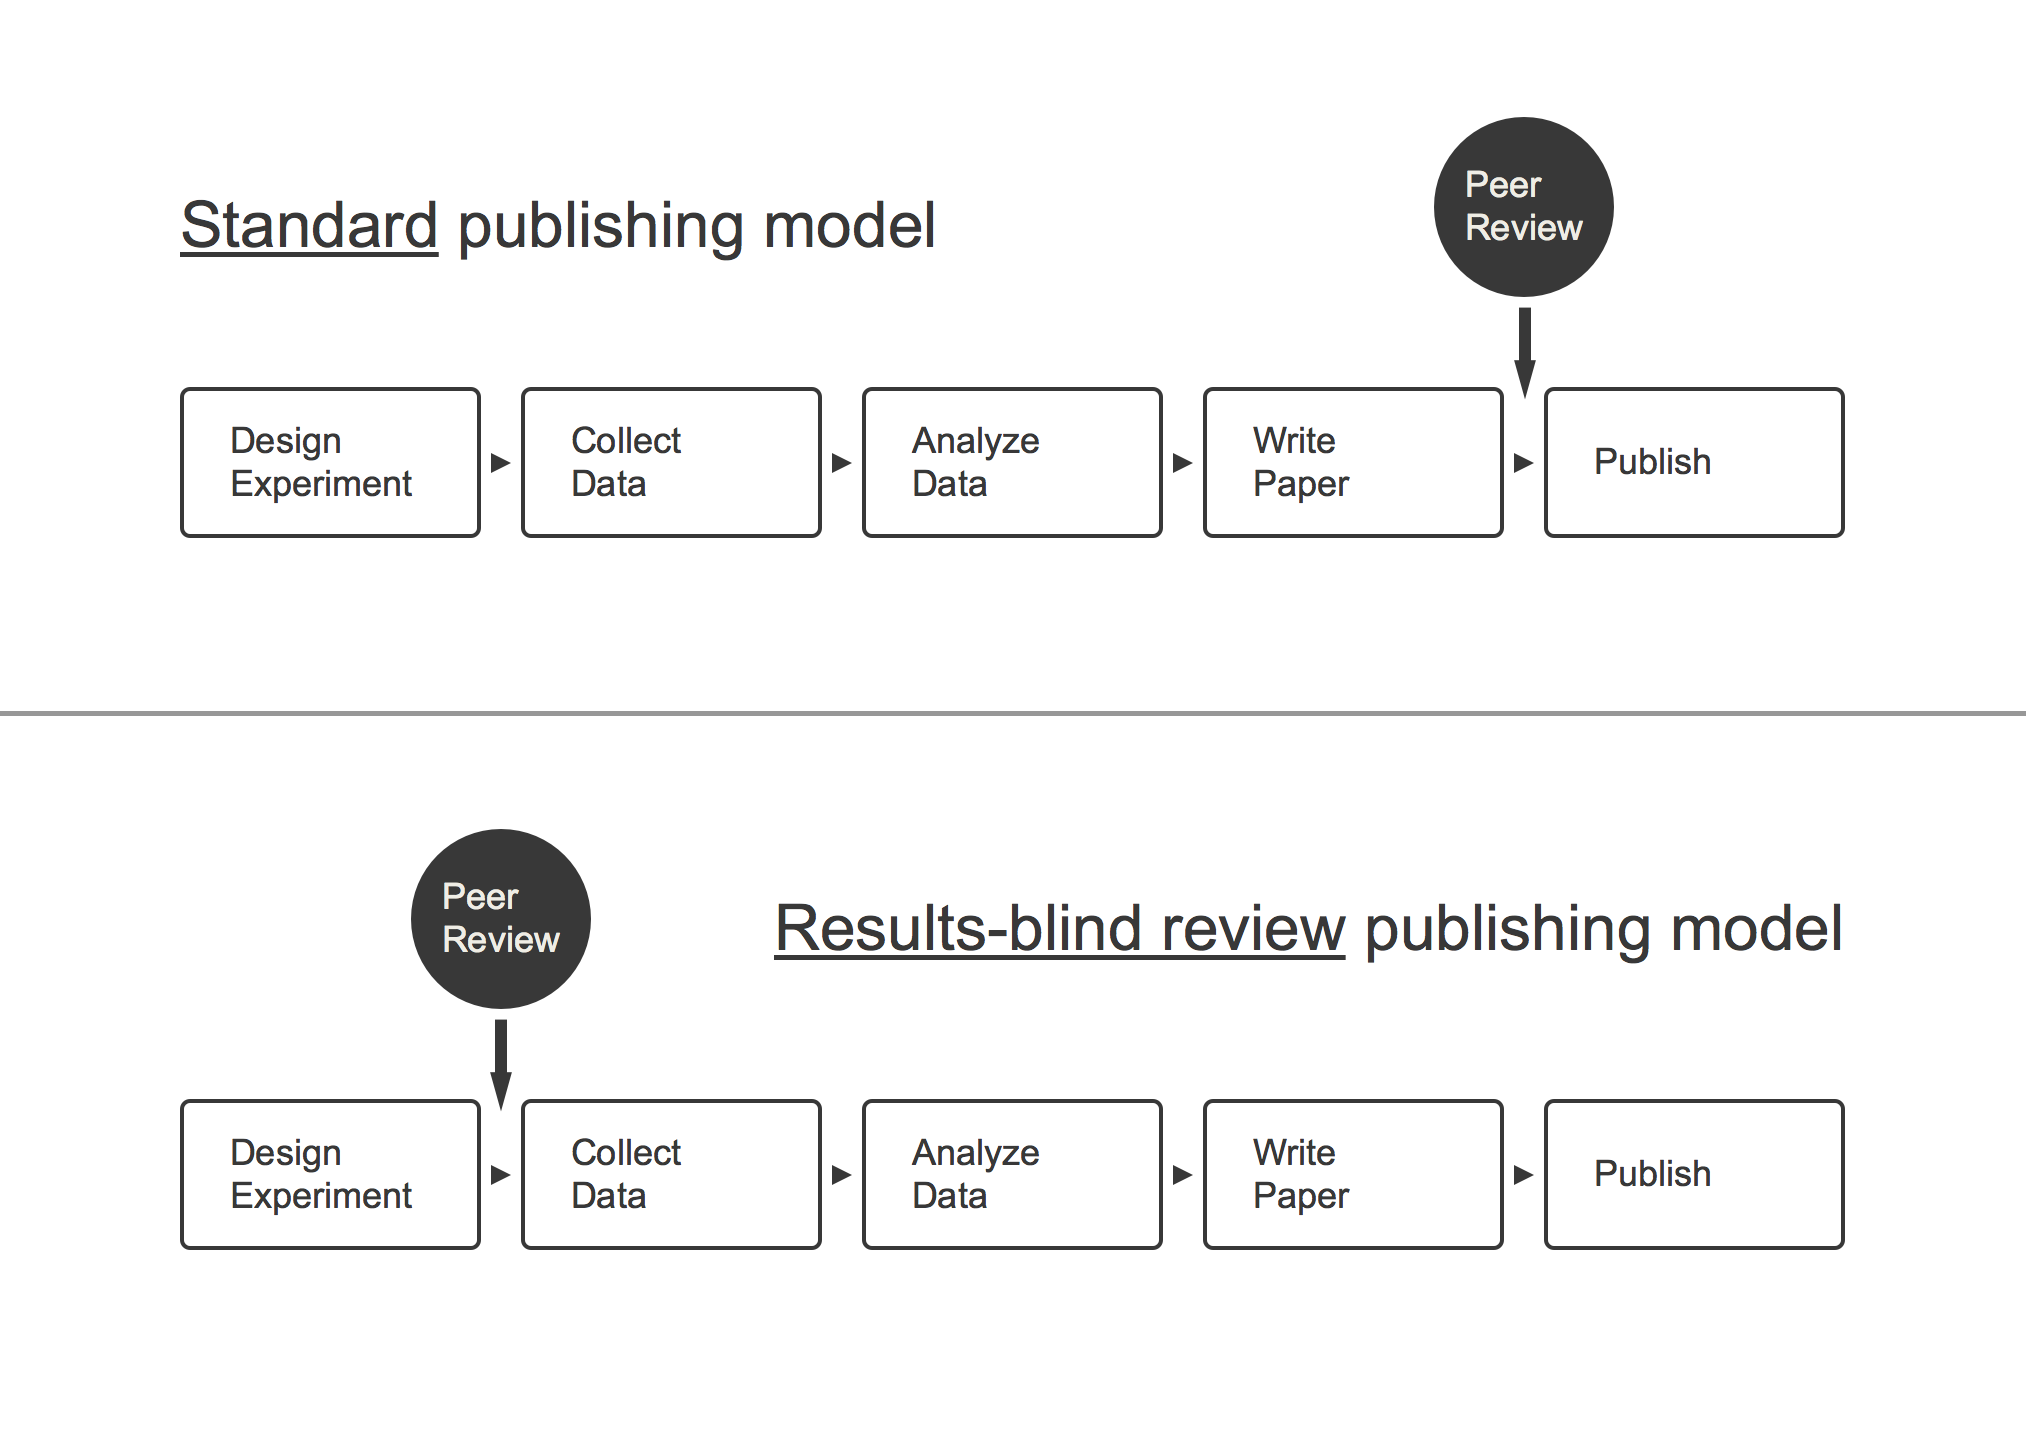
\includegraphics[height=\paperheight]{../Images/results_blind_review.png}
            };
        \end{tikzpicture}
     \end{frame}
}

\begin{frame}{Meta-Analysis}
Synthesize results systematically

\vspace{.2in}
Organizations:
\begin{itemize}[<.->]
\item Cochrane Collaboration (Medicine)
\item Campbell Collaboration (Policy)
\item \href{http://ies.ed.gov/ncee/wwc/}{What Works Clearinghouse (US Gov't, Education)}
\item \href{http://clear.dol.gov/}{CLEAR (US Gov't, Labor)}
\item \href{https://www.hendrix.edu/maer-network/}{MAER-NET} (Economics)
\end{itemize}
\end{frame}

\begin{frame}{Meta-Analysis}
Tools:
\begin{itemize}[<.->]
\item Funnel plots of sample size vs. effect size or precision \href{http://www.jstor.org/stable/2117925}{(Card \& Krueger 1995)}
\item Funnel Asymmetry Test \href{https://books.google.com/books?id=jSQEdEsL7VoC}{(Stanley \& Doucouliagos 2012)}
\item P-curve \href{http://p-curve.com/}{(Simonsohn et al. 2014)} \href{http://p-curve.com/}{\beamergotobutton{Online App}}
\begin{itemize}
	\item One for all P-checker \href{http://shinyapps.org/apps/p-checker/}{\beamergotobutton{Shiny App}}	
\end{itemize}
\end{itemize}
\end{frame}
%%%%%%%%%%%%%%%%%%%%%%%%%%%%%%%%%%%%%%%%%%%%%%%%%%%%%%%%%%%%%%%%%%%%%%%
\section{Pre-Analysis Plans}
\subsection*{P-Hacking}
\begin{frame}[<.->]{P-Hacking}
Define the problem:
\begin{itemize}
\item
Also called fishing, researcher degrees of freedom, or data-mining.
\item
Definition: flexibility in data analysis allows portrayal of \textit{anything} as below an arbitrary p-value threshhold; significance loses its meaning.
\item
Not something only evil people do. It's subconcious, or simply built into statistics (\href{http://www.stat.columbia.edu/~gelman/research/unpublished/p_hacking.pdf}{Gelman, Loken 2013}).
\end{itemize}
\end{frame}

\begin{frame}{P-Hacking is fun!}
\begin{itemize}
\item
``Science isn't Broken'' ---538 journalism piece with interactive demo \href{http://fivethirtyeight.com/features/science-isnt-broken}{\beamerbutton{Link}}
\item 
Train your p-hacking skills R/Shiny App. \href{http://www.nicebread.de/introducing-p-hacker/}{\beamerbutton{Link}}
\item
An Exact Fishy Test \href{https://macartan.shinyapps.io/fish/}{\beamerbutton{Link}}
\end{itemize}
\end{frame}

{ % all template changes are local to this group.
    \setbeamertemplate{navigation symbols}{}
    \begin{frame}[plain]
        \begin{tikzpicture}[remember picture,overlay]
            \node[at=(current page.center)] {
                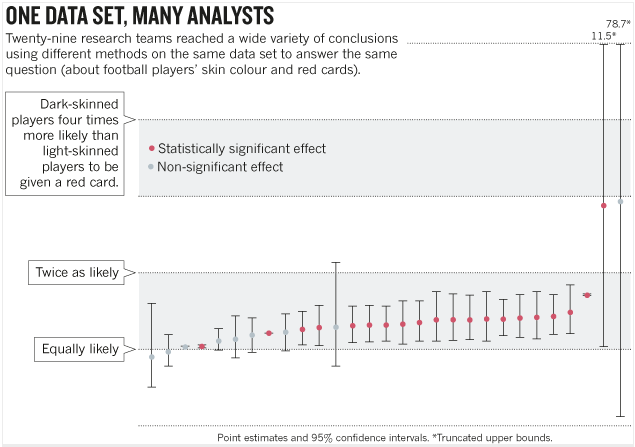
\includegraphics[width=\paperwidth]{../Images/Crowdsourcing2.PNG}
            };
        \end{tikzpicture}
     \end{frame}
}

\subsection*{Pre-Analysis Plan}
\begin{frame}{Pre-Analysis Plan}
Explain the solution:
\begin{itemize}
\item
From 3ie: ``A pre-analysis plan is a detailed description of the analysis to be conducted that is written in advance of seeing the data on impacts of the program being evaluated. It may specify hypotheses to be tested, variable construction, equations to be estimated, controls to be used, and other aspects of the analysis. A key function of the pre-analysis plan is to increase transparency in the research. By setting out the details in advance of what will be done and before knowing the results, the plan guards against data mining and specification searching. Researchers are encouraged to develop and upload such a plan with their study registration, but it is not required for registration.''
\end{itemize}
\end{frame}

\begin{frame}{Origin: FDA's Guidance for Industry}
``E9 Statistical Principles for Clinical Trials'' (1998)
\href{http://www.fda.gov/downloads/drugs/guidancecomplianceregulatoryinformation/guidances/ucm073137.pdf}{\beamergotobutton{Link}}

\S V Data Analysis Considerations
\begin{enumerate}[<.->]
\item Prespecification of the Analysis
\item Analysis Sets
\item Missing Values and Outliers
\item Data Transformation
\item Estimation, Confidence Intervals, and Hypothesis Testing
\item Adjustment of Significance and Confidence Levels
\item Subgroups, Interactions, and Covariates
\item Integrity of Data and Computer Software Validity
\end{enumerate}
\end{frame}


\begin{frame}{Glennerster, Takavarasha Suggestions}
\textit{Running Randomized Evaluations}
\begin{enumerate}[<.->]
\def\labelenumi{\arabic{enumi}.}
\item
  the main outcome measures,
\item
  which outcome measures are primary and which are secondary,
\item
  the precise composition of any families that will be used for mean
  effects analysis,
  \begin{itemize}
  \item Explain mean effects, FWER, FDR using Anderson (\href{https://are.berkeley.edu/~mlanderson/pdf/Anderson\%202008a.pdf}{JASA 2008}).
  \end{itemize}
\item
  the subgroups that will be analyzed,
\item
  the direction of expected impact if we want to use a one-sided test,
  and
\item
  the primary specification to be used for the analysis.
\end{enumerate}
\end{frame}

\begin{frame}{McKenzie Suggestions}
\href{http://blogs.worldbank.org/impactevaluations/a-pre-analysis-plan-checklist}{World Bank Development Impact Blog}

\begin{enumerate}[<.->]
\item
  Description of the sample to be used in the study
\item
  Key data sources
\item
  Hypotheses to be tested throughout the causal chain
\item
  Specify how variables will be constructed
\item
  Specify the treatment effect equation to be estimated
\item
  What is the plan for how to deal with multiple outcomes and multiple
  hypothesis testing?
\item
  Procedures to be used for addressing survey attrition
\item
  How will the study deal with outcomes with limited variation?
\item
  If you are going to be testing a model, include the model
\item
  Remember to archive it
\end{enumerate}
\end{frame}

%\begin{frame}{Simmons, Nelson, Simonsohn (2011)}
%\begin{enumerate}[<.->]
%\def\labelenumi{\arabic{enumi}.}
%\item
%  Authors must decide the rule for terminating data collection before data collection begins and report this rule in the article.
%\item
%  Authors must collect at least 20 observations per cell or else provide
%  a compelling cost-of-data-collection justification.
%\item
%  Authors must list all variables collected in a study.
%\item
%  Authors must report all experimental conditions, including failed
%  manipulations.
%\item
%  If observations are eliminated, authors must also report what the
%  statistical results are if those observations are included.
%\item
%  If an analysis includes a covariate, authors must report the
%  statistical results of the analysis without the covariate.
%\end{enumerate}
%\end{frame}

\begin{frame}{Examples}

\begin{itemize}[<.->]
\item
J-PAL Hypothesis Registry (11), see \url{http://www.povertyactionlab.org/Hypothesis-Registry}

6 published papers:
\begin{itemize}
\item
 Sierra Leone CDD, Oregon Medicare, Turkey Job Training, El Salvador TOMS, two in Indonesia (Olken et al.)
\end{itemize}
\item Psychology: \href{http://pss.sagepub.com/content/26/2/249}{Hawkins, Fitzgerald, Nosek---Conception Risk and Prejudice}
\end{itemize} 
\vspace{0.25in}
Wide range of when exactly to write and how detailed to make the plan. At the extreme level of detail you would have your entire code already written before you got any data.
\end{frame}

{ % all template changes are local to this group.
    \setbeamertemplate{navigation symbols}{}
    \begin{frame}[plain]
         \begin{tikzpicture}[remember picture,overlay]
            \node[at=(current page.center)] {
                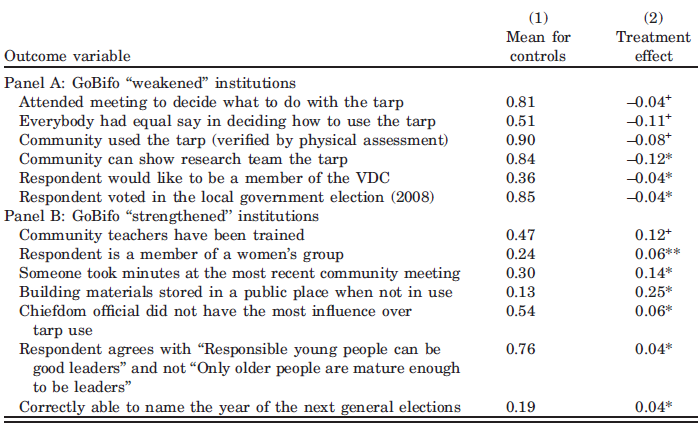
\includegraphics[width=\paperwidth]{../Images/GoBifo1.PNG}
            };
        \end{tikzpicture}
     \end{frame}
}

{ % all template changes are local to this group.
    \setbeamertemplate{navigation symbols}{}
    \begin{frame}[plain]
         \begin{tikzpicture}[remember picture,overlay]
            \node[at=(current page.center)] {
                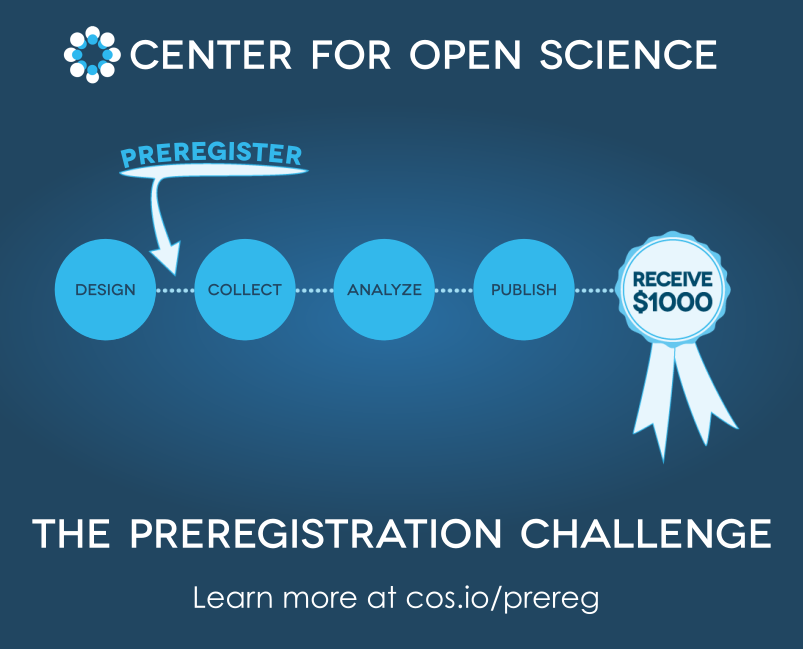
\includegraphics[width=\paperwidth]{../Images/preregchallenge.png}
            };
        \end{tikzpicture}
     \end{frame}
}
%%%%%%%%%%%%%%%%%%%%%%%%%%%%%%%%%%%%%%%%%%%%%%%%%%%%
\begin{frame}{PAP--Observational Studies}
\begin{itemize}[<.->]
\item Debated in public health/epidemiology.
\item Difficult, but not impossible, to verifiably pre-specify.
\item Example: Government data releases
\item Example: Minimum Wage (\href{http://onlinelibrary.wiley.com/doi/10.1111/0019-8676.00199/full}{Neumark 2001})
\end{itemize}
\end{frame}

{ % all template changes are local to this group.
    \setbeamertemplate{navigation symbols}{}
    \begin{frame}[plain]
         \begin{tikzpicture}[remember picture,overlay]
            \node[at=(current page.center)] {
                
\includegraphics[width=\paperwidth]{../Images/Neumark.PNG}
            };
        \end{tikzpicture}
     \end{frame}
}
%%%%%%%%%%%%%%%%%%%%%%%%%%%%%%%%%%%%%%%%%%%%%%%%%%%%%%%%%%%%%%%%%%%%
\section{Replication}
\begin{frame}{Replication}
\begin{enumerate}[<.->]
 \item The Problem	\href{http://www.jstor.org/stable/1806061}{(JMCB Project)}
 \item Project Protocol, Reporting Standards
 \item Organizing Workflow
 \item Code \& Data Sharing
\end{enumerate}
\end{frame}

 { % all template changes are local to this group.
    \setbeamertemplate{navigation symbols}{}
    \begin{frame}[plain, label=AEAreg]
         \begin{tikzpicture}[remember picture,overlay]
            \node[at=(current page.center)] {
                
\includegraphics[width=\paperwidth]{../Images/JMCB1.PNG}
            };
        \end{tikzpicture}
     \end{frame}
}

\subsection*{Project Protocol, Reporting Standards}
\begin{frame}[<.->]{Project Protocol, Reporting Standards}
 Make sure you report everything another researcher would need to replicate your research.
 \begin{itemize}
 \item Find the appropriate reporting standard for your field and follow it: \url{http://www.equator-network.org}
\item Report the nuts and bolts of the project implementation in a detailed protocol: \url{http://www.spirit-statement.org}
\item Transparency and Openness Promotion (TOP) Guidelines: \url{http://cos.io/top}
\end{itemize}
\end{frame}

 { % all template changes are local to this group.
    \setbeamertemplate{navigation symbols}{}
    \begin{frame}[plain, label=AEAreg]
         \begin{tikzpicture}[remember picture,overlay]
            \node[at=(current page.center)] {
                
\includegraphics[width=\paperwidth]{../Images/TOPGuidelines.PNG}
            };
        \end{tikzpicture}
     \end{frame}
}

 \subsection*{Workflow}
 \begin{frame}{Workflow}
``Reproducibility is just collaboration with people you don't know,
including yourself next week''

---Philip Stark, UC Berkeley Statistics
\end{frame}
\begin{frame}{Workflow}

 \begin{itemize}
 \item Practical coding and organizational suggestions
 \begin{itemize}[<.->]
 	\item Making any changes to a file that has been posted/shared means it gets a new name.
 	\item Use version commands to ensure others get same results.
 	\item Long (2008) \textit{The Workflow of Data Analysis Using Stata}
  \end{itemize}
 \item Literate programming (extensive commenting, making the aim of code reading by a human)
 \item Version Control
 \item Dynamic Documents
\end{itemize}
\end{frame}

\subsection*{Version Control}
\begin{frame}{Version Control}
\begin{itemize}[<.->]
\item
Using version control (AKA revision control) can help to make your work more reproducible.

\item
What is version control?

\begin{quote}
Version control is a system that records changes to a file or set of files over time so that you can recall specific versions later. For the examples in this book you will use software source code as the files being version controlled, though in reality you can do this with nearly any type of file on a computer.
\end{quote}
--Git, \href{https://git-scm.com/book/en/v2/Getting-Started-About-Version-Control}{About Version Control}
%\item Distributed Version Control Systems (DCVS) let multiple users control the same files in this manner.
\end{itemize}
\end{frame}

 { % all template changes are local to this group.
    \setbeamertemplate{navigation symbols}{}
    \begin{frame}[plain, label=AEAreg]
         \begin{tikzpicture}[remember picture,overlay]
            \node[at=(current page.center)] {
                
\includegraphics[height=\paperheight]{../Images/github-logo-transparent.JPG}
            };
        \end{tikzpicture}
     \end{frame}

 % all template changes are local to this group.
    \setbeamertemplate{navigation symbols}{}
    \begin{frame}[plain]
         \begin{tikzpicture}[remember picture,overlay]
            \node[at=(current page.center)] {
                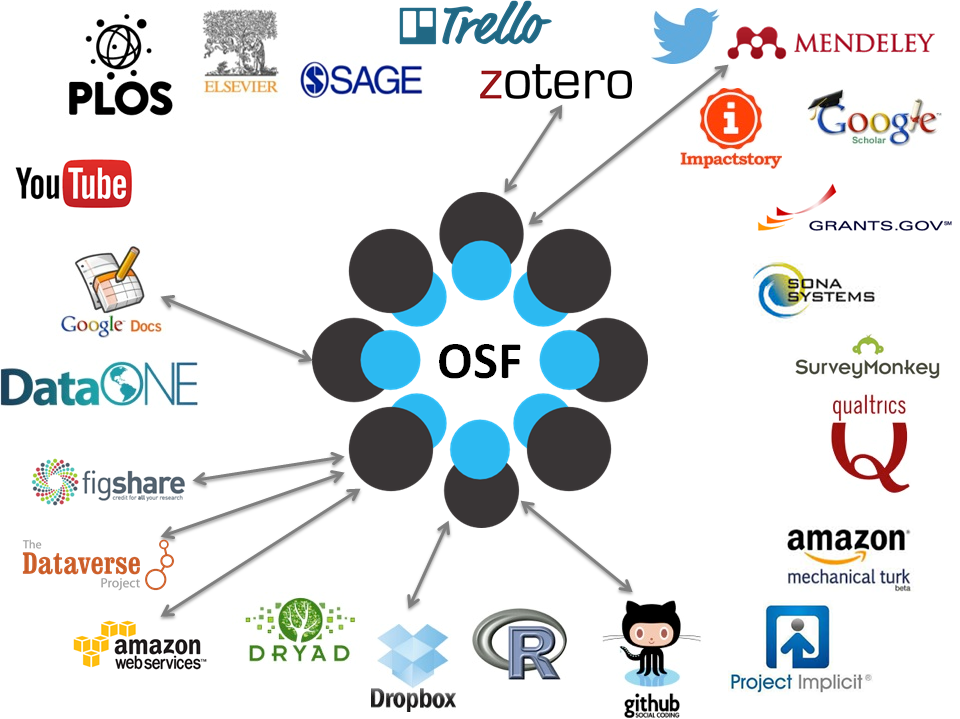
\includegraphics[width=\paperwidth]{../Images/OSFnow.PNG}
            };
        \end{tikzpicture}
     \end{frame}

% all template changes are local to this group.
    \setbeamertemplate{navigation symbols}{}
    \begin{frame}[plain]
         \begin{tikzpicture}[remember picture,overlay]
            \node[at=(current page.center)] {
                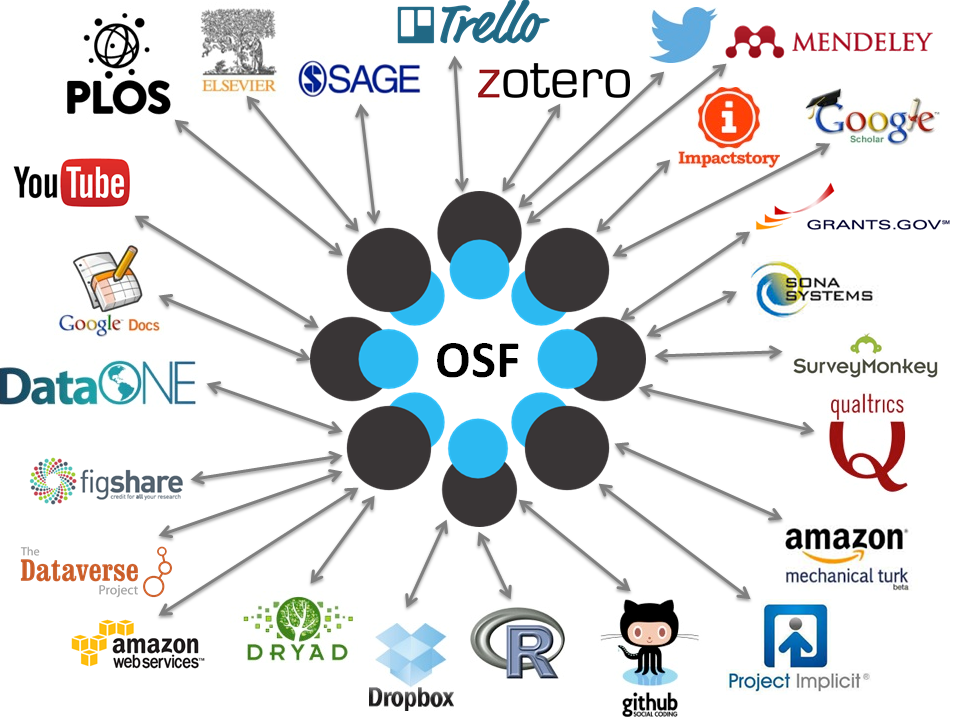
\includegraphics[width=\paperwidth]{../Images/OSFsoon.PNG}
            };
        \end{tikzpicture}
     \end{frame}

}


\begin{frame}{Dynamic Documents}
Write your code and your paper in the same file so you won't lose information or make copy and paste mistakes.

Possible in R and Stata.
\begin{itemize}[<.->]
\item Include tables by linking to a file, instead of a static image.
\item Include number by linking to a value calculated by an analysis file, instead of a static number typed manually.
\item Automatically update tables and numbers.
\item Produce entire paper with one or two clicks.
\end{itemize} 
\end{frame}


 { % all template changes are local to this group.
    \setbeamertemplate{navigation symbols}{}
    \begin{frame}[plain, label=AEAreg]
         \begin{tikzpicture}[remember picture,overlay]
            \node[at=(current page.center)] {
                
\includegraphics[height=\paperheight]{../Images/jupyter.png}
            };
        \end{tikzpicture}
     \end{frame}
}
 { % all template changes are local to this group.
    \setbeamertemplate{navigation symbols}{}
    \begin{frame}[plain, label=AEAreg]
         \begin{tikzpicture}[remember picture,overlay]
            \node[at=(current page.center)] {
                
\includegraphics[width=\paperwidth]{../Images/RStudio-Logo-Blue-Gradient.png}
            };
        \end{tikzpicture}
     \end{frame}
}

\subsection*{Data Sharing}
\begin{frame}{Data Sharing}
Post your code and your data in a trusted public repository.
\begin{itemize}[<.->]
\item
Find the appropriate repository: \url{http://www.re3data.org/}
\item
Repositories will last longer than your own website.
\item
Repositories are more easily searchable by other researchers.
\item
Repositories will store your data in a non-proprietary format that won't become obsolete.
\end{itemize}
\end{frame}

\section{Conclusion}
\begin{frame}{Conclusion}
OK, I'm convinced. How do I implement this in my own research?

\begin{itemize}[<.->]
\item Read the manual I wrote.\href{https://github.com/garretchristensen/BestPracticesManual}{\beamergotobutton{Link}}
\item Subscribe to the BITSS blog \& E-mail list \href{https://bitss.org/blog}{\beamergotobutton{Link}}
\item Apply for our NIH Summer Institute. \href{http://www.bitss.org/events/summer-institute/}{\beamergotobutton{Link}}
\item Apply for our SSMART Grants (extra funding for developing country researchers). \href{http://www.bitss.org/ssmart-grants/}{\beamergotobutton{Link}}
\item Apply for our Leamer-Rosenthal Prizes. \href{http://www.bitss.org/lr-prizes/}{\beamergotobutton{Link}}
\item Free stats consulting from COS. \href{https://cos.io/stats_consulting/}{\beamergotobutton{Link}}
\end{itemize}
\end{frame}

\begin{frame}{Summer Institute}
Three days of training in June at UC Berkeley, or two days of training in July at the University of Michigan.
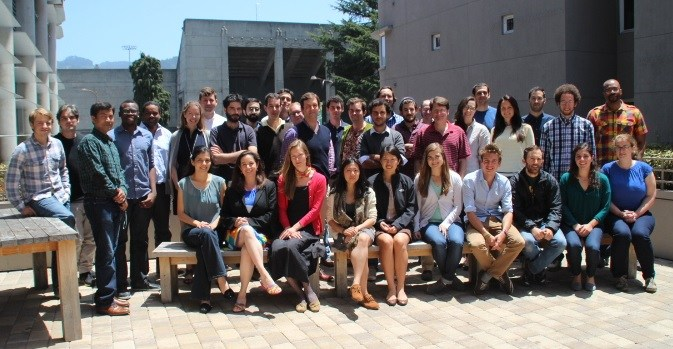
\includegraphics[width=4in]{../Images/bitss-2014-cohort2.jpg}
\end{frame}

\begin{frame}{SSMART Grant}
Up to \$30,000 grant for a research project on:
\begin{itemize}[<.->]
\item Develop new methodology
\item New tools and approaches for meta-analysis
\item Research on researchers and adoption of new norms
\end{itemize}
Extra funding source for researchers from developing countries.

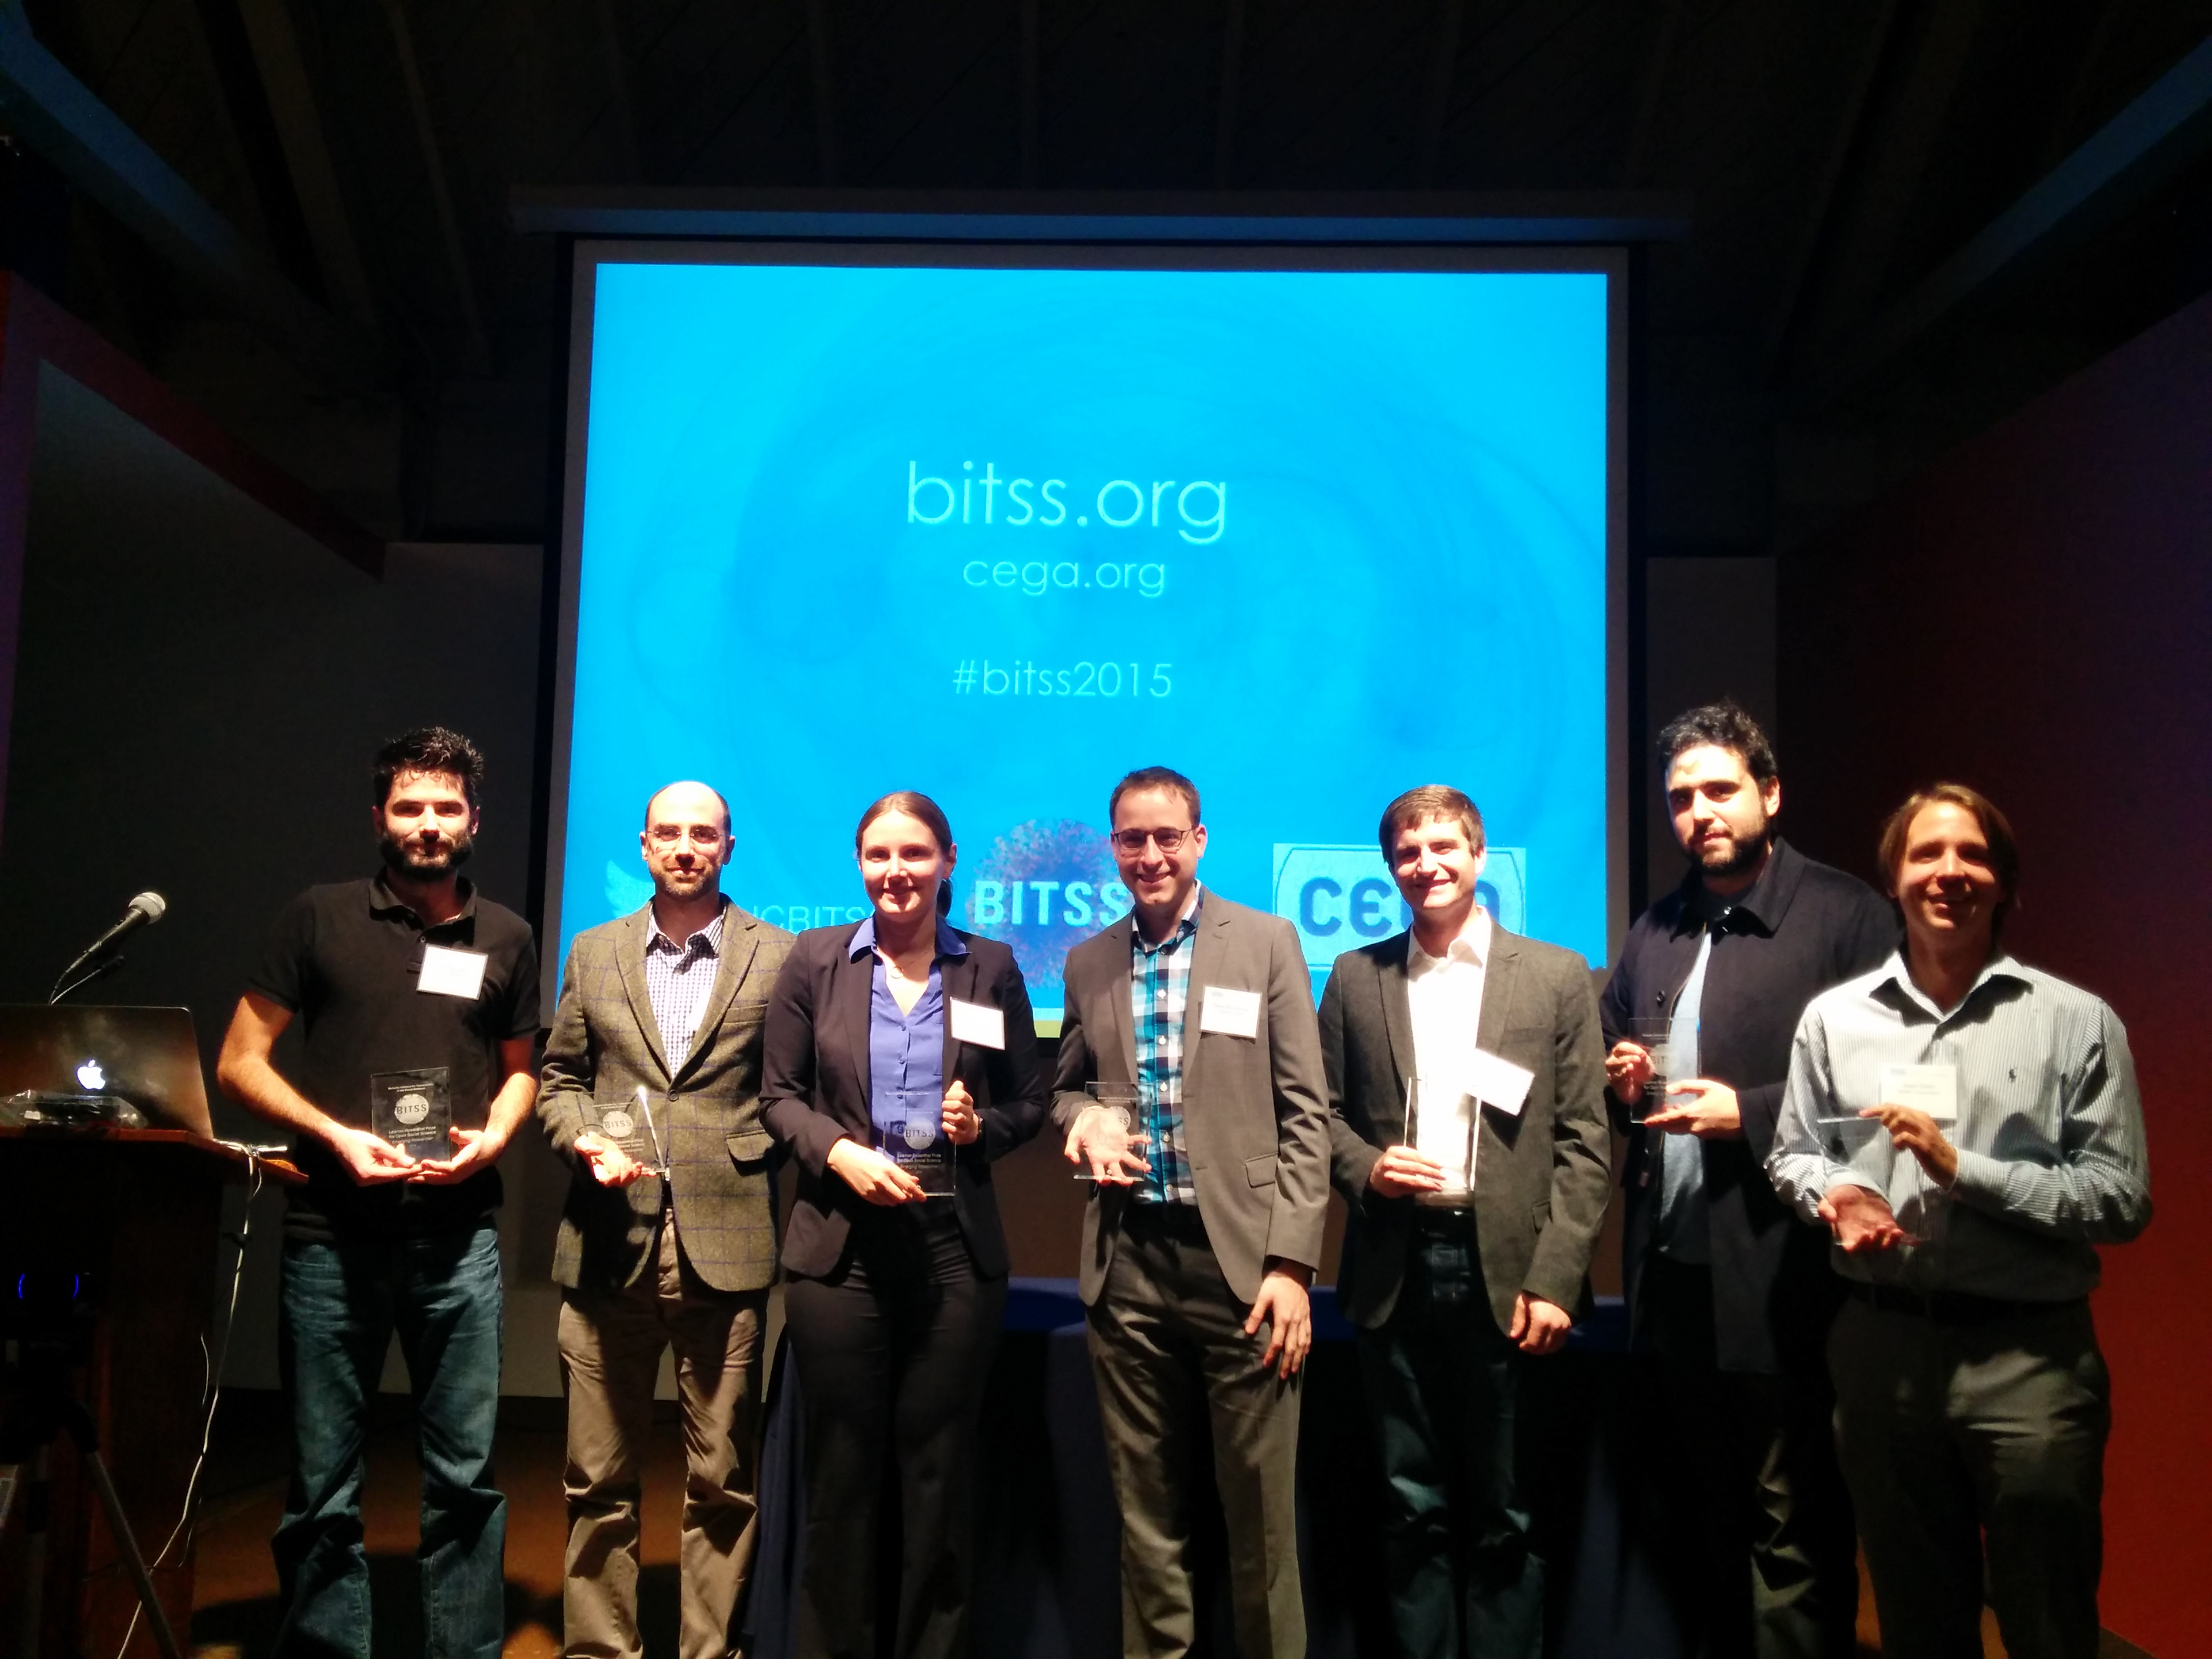
\includegraphics[width=2.5in]{../Images/LRwinners.jpg}
\end{frame}

\begin{frame}{Leamer-Rosenthal Prizes}
Up to \$10,000 prize for completed transparent research in the social sciences,
especially:
\begin{itemize}[<.->]
\item Economics
\item Political Science
\item Psychology
\end{itemize}
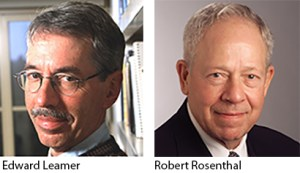
\includegraphics[width=2.5in]{../Images/leamer1-zoomed33.jpg}
\end{frame}


\begin{frame}
\begin{center}
Questions?
\vspace{1in}


\Huge{Thank you!}
\end{center}
\end{frame}

\end{document}

